\begin{enumerate}[label=\thechapter.\arabic*,ref=\thechapter.\theenumi]
\numberwithin{equation}{enumi}
\numberwithin{figure}{enumi}
\numberwithin{table}{enumi}

  \item The point on the curve 
    \begin{align}
        x^2 = 2y
        \label{eq:12/6/5/27/nonconv/lagmul/curve}
    \end{align}
    which is nearest to the point 
    $\vec{P} = \myvec{0\\5}$ is
    \begin{enumerate}
        \item $\myvec{2\sqrt{2}\\4}$
        \item $\myvec{2\sqrt{2}\\0}$
        \item $\myvec{0\\0}$
        \item $\myvec{2\\2}$
    \end{enumerate}
\solution 
		\begin{enumerate}
	\item Optimization Problem
		\\
	\item  Gradient Descent
		\\
\label{12/6/5/27/nonconv/grad}
\iffalse
\documentclass[journal,12pt,twocolumn]{IEEEtran}
\usepackage{setspace}
\usepackage{gensymb}
\usepackage{xcolor}
\usepackage{caption}
\singlespacing
\usepackage{siunitx}
\usepackage[cmex10]{amsmath}
\usepackage{mathtools}
\usepackage{hyperref}
\usepackage{amsthm}
\usepackage{mathrsfs}
\usepackage{txfonts}
\usepackage{stfloats}
\usepackage{cite}
\usepackage{cases}
\usepackage{subfig}
\usepackage{longtable}
\usepackage{multirow}
\usepackage{enumitem}
\usepackage{bm}
\usepackage{mathtools}
\usepackage{listings}
\usepackage{tikz}
\usetikzlibrary{shapes,arrows,positioning}
\usepackage{circuitikz}
\renewcommand{\vec}[1]{\boldsymbol{\mathbf{#1}}}
\DeclareMathOperator*{\Res}{Res}
\renewcommand\thesection{\arabic{section}}
\renewcommand\thesubsection{\thesection.\arabic{subsection}}
\renewcommand\thesubsubsection{\thesubsection.\arabic{subsubsection}}

\renewcommand\thesectiondis{\arabic{section}}
\renewcommand\thesubsectiondis{\thesectiondis.\arabic{subsection}}
\renewcommand\thesubsubsectiondis{\thesubsectiondis.\arabic{subsubsection}}
\hyphenation{op-tical net-works semi-conduc-tor}

\lstset{
language=Python,
frame=single, 
breaklines=true,
columns=fullflexible
}
\begin{document}
\theoremstyle{definition}
\newtheorem{theorem}{Theorem}[section]
\newtheorem{problem}{Problem}
\newtheorem{proposition}{Proposition}[section]
\newtheorem{lemma}{Lemma}[section]
\newtheorem{corollary}[theorem]{Corollary}
\newtheorem{example}{Example}[section]
\newtheorem{definition}{Definition}[section]
\newcommand{\BEQA}{\begin{eqnarray}}
\newcommand{\EEQA}{\end{eqnarray}}
\newcommand{\define}{\stackrel{\triangle}{=}}
\newcommand{\myvec}[1]{\ensuremath{\begin{pmatrix}#1\end{pmatrix}}}
\newcommand{\mydet}[1]{\ensuremath{\begin{vmatrix}#1\end{vmatrix}}}
\bibliographystyle{IEEEtran}
\providecommand{\nCr}[2]{\,^{#1}C_{#2}} % nCr
\providecommand{\nPr}[2]{\,^{#1}P_{#2}} % nPr
\providecommand{\mbf}{\mathbf}
\providecommand{\pr}[1]{\ensuremath{\Pr\left(#1\right)}}
\providecommand{\qfunc}[1]{\ensuremath{Q\left(#1\right)}}
\providecommand{\sbrak}[1]{\ensuremath{{}\left[#1\right]}}
\providecommand{\lsbrak}[1]{\ensuremath{{}\left[#1\right.}}
\providecommand{\rsbrak}[1]{\ensuremath{{}\left.#1\right]}}
\providecommand{\brak}[1]{\ensuremath{\left(#1\right)}}
\providecommand{\lbrak}[1]{\ensuremath{\left(#1\right.}}
\providecommand{\rbrak}[1]{\ensuremath{\left.#1\right)}}
\providecommand{\cbrak}[1]{\ensuremath{\left\{#1\right\}}}
\providecommand{\lcbrak}[1]{\ensuremath{\left\{#1\right.}}
\providecommand{\rcbrak}[1]{\ensuremath{\left.#1\right\}}}
\theoremstyle{remark}
\newtheorem{rem}{Remark}
\newcommand{\sgn}{\mathop{\mathrm{sgn}}}
\newcommand{\rect}{\mathop{\mathrm{rect}}}
\newcommand{\sinc}{\mathop{\mathrm{sinc}}}
\providecommand{\abs}[1]{\left\vert#1\right\vert}
\providecommand{\res}[1]{\Res\displaylimits_{#1}} 
\providecommand{\norm}[1]{\left\Vert#1\right\Vert}
\providecommand{\mtx}[1]{\mathbf{#1}}
\providecommand{\mean}[1]{E\left[ #1 \right]}
\providecommand{\fourier}{\overset{\mathcal{F}}{ \rightleftharpoons}}
\providecommand{\ztrans}{\overset{\mathcal{Z}}{ \rightleftharpoons}}
\providecommand{\system}[1]{\overset{\mathcal{#1}}{ \longleftrightarrow}}
\newcommand{\solution}{\noindent \textbf{Solution: }}
\providecommand{\dec}[2]{\ensuremath{\overset{#1}{\underset{#2}{\gtrless}}}}
\let\StandardTheFigure\thefigure
\def\putbox#1#2#3{\makebox[0in][l]{\makebox[#1][l]{}\raisebox{\baselineskip}[0in][0in]{\raisebox{#2}[0in][0in]{#3}}}}
     \def\rightbox#1{\makebox[0in][r]{#1}}
     \def\centbox#1{\makebox[0in]{#1}}
     \def\topbox#1{\raisebox{-\baselineskip}[0in][0in]{#1}}
     \def\midbox#1{\raisebox{-0.5\baselineskip}[0in][0in]{#1}}

\vspace{3cm}
\title{Quadratic Programming Assignment}
\author{Gautam Singh}
\maketitle
\bigskip

\begin{abstract}
    This document contains the solution to Question 27 of Exercise 5 in Chapter
    6 of the class 12 NCERT textbook.
\end{abstract}

\begin{enumerate}
  
    \solution 
    \fi
		We need to find
    \begin{align}
        \min_{\vec{x}} g\brak{\vec{x}} &= \norm{\vec{x}-\vec{P}}^2 \label{eq:12/6/5/27/nonconv/grad/cost} \\
        \textrm{s.t. } h\brak{\vec{x}} &= \vec{x}^\top\vec{Vx} + 2\vec{u}^\top\vec{x} = 0 \label{eq:12/6/5/27/nonconv/grad/constr}
    \end{align}
    where
    \begin{align}
        \vec{V} = \myvec{1&0\\0&0},\ \vec{u} = \myvec{0\\-1}
    \end{align}
    We find the required minima using constrained gradient descent in 
    Fig. \ref{fig:12/6/5/27/nonconv/grad/gd-pits}, plotted using the Python code 
    \texttt{codes/grad\_pits.py}.
    \begin{figure}[!ht]
        \centering
        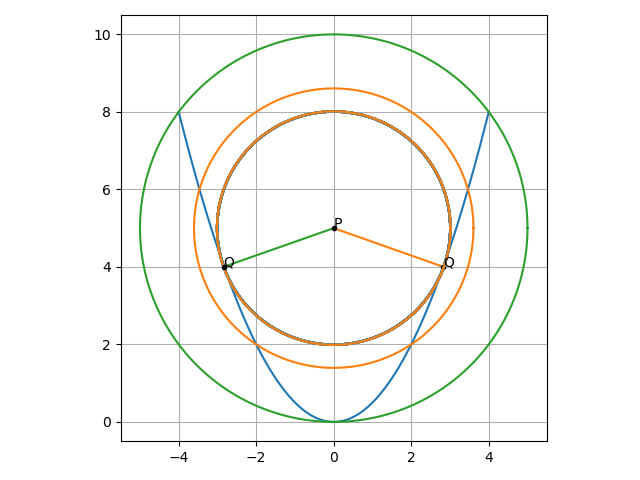
\includegraphics[width=\columnwidth]{12/6/5/27/nonconv/grad/figs/grad_pits.png}
        \caption{Gradient descent for a nonconvex optimization problem.}
        \label{fig:12/6/5/27/nonconv/grad/gd-pits}
    \end{figure}

\item Convex Constraint
	\\
\label{12/6/5/27/conv/grad}
\iffalse
\documentclass[journal,12pt,twocolumn]{IEEEtran}
\usepackage{setspace}
\usepackage{gensymb}
\usepackage{xcolor}
\usepackage{caption}
\singlespacing
\usepackage{siunitx}
\usepackage[cmex10]{amsmath}
\usepackage{mathtools}
\usepackage{hyperref}
\usepackage{amsthm}
\usepackage{mathrsfs}
\usepackage{txfonts}
\usepackage{stfloats}
\usepackage{cite}
\usepackage{cases}
\usepackage{subfig}
\usepackage{longtable}
\usepackage{multirow}
\usepackage{enumitem}
\usepackage{bm}
\usepackage{mathtools}
\usepackage{listings}
\usepackage{tikz}
\usetikzlibrary{shapes,arrows,positioning}
\usepackage{circuitikz}
\renewcommand{\vec}[1]{\boldsymbol{\mathbf{#1}}}
\DeclareMathOperator*{\Res}{Res}
\renewcommand\thesection{\arabic{section}}
\renewcommand\thesubsection{\thesection.\arabic{subsection}}
\renewcommand\thesubsubsection{\thesubsection.\arabic{subsubsection}}

\renewcommand\thesectiondis{\arabic{section}}
\renewcommand\thesubsectiondis{\thesectiondis.\arabic{subsection}}
\renewcommand\thesubsubsectiondis{\thesubsectiondis.\arabic{subsubsection}}
\hyphenation{op-tical net-works semi-conduc-tor}

\lstset{
language=Python,
frame=single, 
breaklines=true,
columns=fullflexible
}
\begin{document}
\theoremstyle{definition}
\newtheorem{theorem}{Theorem}[section]
\newtheorem{problem}{Problem}
\newtheorem{proposition}{Proposition}[section]
\newtheorem{lemma}{Lemma}[section]
\newtheorem{corollary}[theorem]{Corollary}
\newtheorem{example}{Example}[section]
\newtheorem{definition}{Definition}[section]
\newcommand{\BEQA}{\begin{eqnarray}}
\newcommand{\EEQA}{\end{eqnarray}}
\newcommand{\define}{\stackrel{\triangle}{=}}
\newcommand{\myvec}[1]{\ensuremath{\begin{pmatrix}#1\end{pmatrix}}}
\newcommand{\mydet}[1]{\ensuremath{\begin{vmatrix}#1\end{vmatrix}}}
\bibliographystyle{IEEEtran}
\providecommand{\nCr}[2]{\,^{#1}C_{#2}} % nCr
\providecommand{\nPr}[2]{\,^{#1}P_{#2}} % nPr
\providecommand{\mbf}{\mathbf}
\providecommand{\pr}[1]{\ensuremath{\Pr\left(#1\right)}}
\providecommand{\qfunc}[1]{\ensuremath{Q\left(#1\right)}}
\providecommand{\sbrak}[1]{\ensuremath{{}\left[#1\right]}}
\providecommand{\lsbrak}[1]{\ensuremath{{}\left[#1\right.}}
\providecommand{\rsbrak}[1]{\ensuremath{{}\left.#1\right]}}
\providecommand{\brak}[1]{\ensuremath{\left(#1\right)}}
\providecommand{\lbrak}[1]{\ensuremath{\left(#1\right.}}
\providecommand{\rbrak}[1]{\ensuremath{\left.#1\right)}}
\providecommand{\cbrak}[1]{\ensuremath{\left\{#1\right\}}}
\providecommand{\lcbrak}[1]{\ensuremath{\left\{#1\right.}}
\providecommand{\rcbrak}[1]{\ensuremath{\left.#1\right\}}}
\theoremstyle{remark}
\newtheorem{rem}{Remark}
\newcommand{\sgn}{\mathop{\mathrm{sgn}}}
\newcommand{\rect}{\mathop{\mathrm{rect}}}
\newcommand{\sinc}{\mathop{\mathrm{sinc}}}
\providecommand{\abs}[1]{\left\vert#1\right\vert}
\providecommand{\res}[1]{\Res\displaylimits_{#1}} 
\providecommand{\norm}[1]{\left\Vert#1\right\Vert}
\providecommand{\mtx}[1]{\mathbf{#1}}
\providecommand{\mean}[1]{E\left[ #1 \right]}
\providecommand{\fourier}{\overset{\mathcal{F}}{ \rightleftharpoons}}
\providecommand{\ztrans}{\overset{\mathcal{Z}}{ \rightleftharpoons}}
\providecommand{\system}[1]{\overset{\mathcal{#1}}{ \longleftrightarrow}}
\newcommand{\solution}{\noindent \textbf{Solution: }}
\providecommand{\dec}[2]{\ensuremath{\overset{#1}{\underset{#2}{\gtrless}}}}
\let\StandardTheFigure\thefigure
\def\putbox#1#2#3{\makebox[0in][l]{\makebox[#1][l]{}\raisebox{\baselineskip}[0in][0in]{\raisebox{#2}[0in][0in]{#3}}}}
     \def\rightbox#1{\makebox[0in][r]{#1}}
     \def\centbox#1{\makebox[0in]{#1}}
     \def\topbox#1{\raisebox{-\baselineskip}[0in][0in]{#1}}
     \def\midbox#1{\raisebox{-0.5\baselineskip}[0in][0in]{#1}}

\vspace{3cm}
\title{Quadratic Programming Assignment}
\author{Gautam Singh}
\maketitle
\bigskip

\begin{abstract}
    This document contains the solution to a modification to Question 27 of 
    Exercise 5 in Chapter 6 of the class 12 NCERT textbook.
\end{abstract}

\begin{enumerate}
      \solution 
\fi
		We need to find
    \begin{align}
        \min_{\vec{x}} g\brak{\vec{x}} &= \norm{\vec{x}-\vec{P}}^2 \label{eq:12/6/5/27/conv/gradcost} \\
        \textrm{s.t. } h\brak{\vec{x}} &= \vec{x}^\top\vec{Vx} + 2\vec{u}^\top\vec{x} = 0 \label{eq:12/6/5/27/conv/gradconstr}
    \end{align}
    where
    \begin{align}
        \vec{V} = \myvec{1&0\\0&0},\ \vec{u} = \myvec{0\\-1}
    \end{align}

    We find the required minima using constrained gradient descent in 
    Fig. \ref{fig:12/6/5/27/conv/gradgd-pits}, plotted using Python.
    \begin{figure}[!ht]
        \centering
        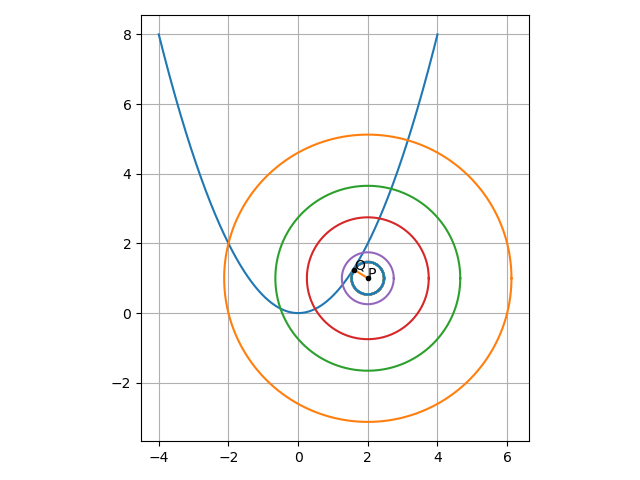
\includegraphics[width=\columnwidth]{12/6/5/27/conv/grad/figs/grad_pits.png}
        \caption{Gradient descent for a convex optimization problem.}
        \label{fig:12/6/5/27/conv/gradgd-pits}
    \end{figure}

\item  Lagrange Multipliers
	\\
\label{12/6/5/27/nonconv/lagmul}
\iffalse
\documentclass[journal,12pt,twocolumn]{IEEEtran}
\usepackage{setspace}
\usepackage{gensymb}
\usepackage{xcolor}
\usepackage{caption}
\singlespacing
\usepackage{siunitx}
\usepackage[cmex10]{amsmath}
\usepackage{mathtools}
\usepackage{hyperref}
\usepackage{amsthm}
\usepackage{mathrsfs}
\usepackage{txfonts}
\usepackage{stfloats}
\usepackage{cite}
\usepackage{cases}
\usepackage{subfig}
\usepackage{longtable}
\usepackage{multirow}
\usepackage{enumitem}
\usepackage{bm}
\usepackage{mathtools}
\usepackage{listings}
\usepackage{tikz}
\usetikzlibrary{shapes,arrows,positioning}
\usepackage{circuitikz}
\renewcommand{\vec}[1]{\boldsymbol{\mathbf{#1}}}
\DeclareMathOperator*{\Res}{Res}
\renewcommand\thesection{\arabic{section}}
\renewcommand\thesubsection{\thesection.\arabic{subsection}}
\renewcommand\thesubsubsection{\thesubsection.\arabic{subsubsection}}

\renewcommand\thesectiondis{\arabic{section}}
\renewcommand\thesubsectiondis{\thesectiondis.\arabic{subsection}}
\renewcommand\thesubsubsectiondis{\thesubsectiondis.\arabic{subsubsection}}
\hyphenation{op-tical net-works semi-conduc-tor}

\lstset{
language=Python,
frame=single, 
breaklines=true,
columns=fullflexible
}
\begin{document}
\theoremstyle{definition}
\newtheorem{theorem}{Theorem}[section]
\newtheorem{problem}{Problem}
\newtheorem{proposition}{Proposition}[section]
\newtheorem{lemma}{Lemma}[section]
\newtheorem{corollary}[theorem]{Corollary}
\newtheorem{example}{Example}[section]
\newtheorem{definition}{Definition}[section]
\newcommand{\BEQA}{\begin{eqnarray}}
\newcommand{\EEQA}{\end{eqnarray}}
\newcommand{\define}{\stackrel{\triangle}{=}}
\newcommand{\myvec}[1]{\ensuremath{\begin{pmatrix}#1\end{pmatrix}}}
\newcommand{\mydet}[1]{\ensuremath{\begin{vmatrix}#1\end{vmatrix}}}
\bibliographystyle{IEEEtran}
\providecommand{\nCr}[2]{\,^{#1}C_{#2}} % nCr
\providecommand{\nPr}[2]{\,^{#1}P_{#2}} % nPr
\providecommand{\mbf}{\mathbf}
\providecommand{\pr}[1]{\ensuremath{\Pr\left(#1\right)}}
\providecommand{\qfunc}[1]{\ensuremath{Q\left(#1\right)}}
\providecommand{\sbrak}[1]{\ensuremath{{}\left[#1\right]}}
\providecommand{\lsbrak}[1]{\ensuremath{{}\left[#1\right.}}
\providecommand{\rsbrak}[1]{\ensuremath{{}\left.#1\right]}}
\providecommand{\brak}[1]{\ensuremath{\left(#1\right)}}
\providecommand{\lbrak}[1]{\ensuremath{\left(#1\right.}}
\providecommand{\rbrak}[1]{\ensuremath{\left.#1\right)}}
\providecommand{\cbrak}[1]{\ensuremath{\left\{#1\right\}}}
\providecommand{\lcbrak}[1]{\ensuremath{\left\{#1\right.}}
\providecommand{\rcbrak}[1]{\ensuremath{\left.#1\right\}}}
\theoremstyle{remark}
\newtheorem{rem}{Remark}
\newcommand{\sgn}{\mathop{\mathrm{sgn}}}
\newcommand{\rect}{\mathop{\mathrm{rect}}}
\newcommand{\sinc}{\mathop{\mathrm{sinc}}}
\providecommand{\abs}[1]{\left\vert#1\right\vert}
\providecommand{\res}[1]{\Res\displaylimits_{#1}} 
\providecommand{\norm}[1]{\left\Vert#1\right\Vert}
\providecommand{\mtx}[1]{\mathbf{#1}}
\providecommand{\mean}[1]{E\left[ #1 \right]}
\providecommand{\fourier}{\overset{\mathcal{F}}{ \rightleftharpoons}}
\providecommand{\ztrans}{\overset{\mathcal{Z}}{ \rightleftharpoons}}
\providecommand{\system}[1]{\overset{\mathcal{#1}}{ \longleftrightarrow}}
\newcommand{\solution}{\noindent \textbf{Solution: }}
\providecommand{\dec}[2]{\ensuremath{\overset{#1}{\underset{#2}{\gtrless}}}}
\let\StandardTheFigure\thefigure
\def\putbox#1#2#3{\makebox[0in][l]{\makebox[#1][l]{}\raisebox{\baselineskip}[0in][0in]{\raisebox{#2}[0in][0in]{#3}}}}
     \def\rightbox#1{\makebox[0in][r]{#1}}
     \def\centbox#1{\makebox[0in]{#1}}
     \def\topbox#1{\raisebox{-\baselineskip}[0in][0in]{#1}}
     \def\midbox#1{\raisebox{-0.5\baselineskip}[0in][0in]{#1}}

\vspace{3cm}
\title{Quadratic Programming Assignment}
\author{Gautam Singh}
\maketitle
\bigskip

\begin{abstract}
    This document contains the solution to Question 27 of Exercise 5 in Chapter
    6 of the class 12 NCERT textbook.
\end{abstract}

\begin{enumerate}
  
    \solution 
    \fi
		We need to find
    \begin{align}
        \min_{\vec{x}} g\brak{\vec{x}} &= \norm{\vec{x}-\vec{P}}^2 \label{eq:12/6/5/27/nonconv/lagmul/cost} \\
        \textrm{s.t. } h\brak{\vec{x}} &= \vec{x}^\top\vec{Vx} + 2\vec{u}^\top\vec{x} = 0 \label{eq:12/6/5/27/nonconv/lagmul/constr}
    \end{align}
    where
    \begin{align}
        \vec{V} = \myvec{1&0\\0&0},\ \vec{u} = \myvec{0\\-1}
    \end{align}

    Since the given optimization problem is nonconvex, we use the method of 
    Lagrange multipliers to find the optima. Here, we need to find 
    $\lambda \in \mathbb{R}$ such that there exists a $\vec{x}$ 
    satisfying
    \begin{align}
        \nabla g\brak{\vec{x}} &= \lambda\nabla h\brak{\vec{x}} \\
        \implies 2\brak{\vec{x}-\vec{P}} &= 2\lambda\brak{\vec{Ax}+\vec{u}} \\
        \implies \brak{\vec{I}-\lambda\vec{A}}\vec{x} &= \lambda\vec{u} + \vec{P} \\
        \implies \myvec{1-\lambda&0\\0&1}\vec{x} &= \myvec{0\\5-\lambda}
        \label{eq:12/6/5/27/nonconv/lagmul/lagmul}
    \end{align}
    From \eqref{eq:12/6/5/27/nonconv/lagmul/lagmul}, we have two cases:
    \begin{enumerate}
        \item $\lambda \neq 1$. In this case, we form the augmented matrix
        \begin{align}
            \myvec{1-\lambda&0&0\\0&1&5-\lambda} \xleftrightarrow[]{R_1 \leftarrow \frac{R_1}{1-\lambda}} \myvec{1&0&0\\0&1&5-\lambda}
        \end{align}
        and get that
        \begin{align}
            \vec{x_m} = \myvec{0\\5-\lambda}
        \end{align}
        Substituting in \eqref{eq:12/6/5/27/nonconv/lagmul/constr} gives $\lambda = 5$. Thus, 
        $\vec{x_m} = \vec{0}$.

        \item $\lambda = 1$. In this case, \eqref{eq:12/6/5/27/nonconv/lagmul/lagmul} becomes
        \begin{align}
            \myvec{0&0\\0&1}\vec{x} &= \myvec{0\\4} \\
            \implies \vec{e_2}^\top\vec{x} = 4
            \label{eq:12/6/5/27/nonconv/lagmul/x-e2}
        \end{align}
        Substituting \eqref{eq:12/6/5/27/nonconv/lagmul/x-e2} into \eqref{eq:12/6/5/27/nonconv/lagmul/constr} becomes
        \begin{align}
            \brak{\vec{e_1}^\top\vec{x}}^2 &= 8 \\
            \implies \vec{e_1}^\top\vec{x} &= \pm 2\sqrt{2}
            \label{eq:12/6/5/27/nonconv/lagmul/x-e1}
        \end{align}
        Using \eqref{eq:12/6/5/27/nonconv/lagmul/x-e1} and \eqref{eq:12/6/5/27/nonconv/lagmul/x-e2},
        \begin{align}
            \vec{x_m} = \myvec{\pm 2\sqrt{2}\\4}
        \end{align}
    \end{enumerate}
    Using these values of $\vec{x_m}$, the distances are
    \begin{align}
        \norm{\myvec{0\\5}-\myvec{0\\0}} &= 5 \\
        \norm{\myvec{0\\5}-\myvec{\pm 2\sqrt{2}\\4}} &= 3
        \label{eq:12/6/5/27/nonconv/lagmul/true-min}
    \end{align}
    Thus, the correct answer is \textbf{a)}.

		\end{enumerate}
 \item Find the point on the curve 
    \begin{align}
        x^2 = 2y
        \label{eq:curve}
        %\label{eq:12/6/5/27/conv/conv/curve}
    \end{align}
    which is nearest to the point $\vec{P} = \myvec{2\\1}$.
    \\
\solution 
		\begin{enumerate}
			\item Quadratic Progamming
				\\
\label{12/6/5/27/conv/conv}
\iffalse
\documentclass[journal,12pt,twocolumn]{IEEEtran}
\usepackage{setspace}
\usepackage{gensymb}
\usepackage{xcolor}
\usepackage{caption}
\singlespacing
\usepackage{siunitx}
\usepackage[cmex10]{amsmath}
\usepackage{mathtools}
\usepackage{hyperref}
\usepackage{amsthm}
\usepackage{mathrsfs}
\usepackage{txfonts}
\usepackage{stfloats}
\usepackage{cite}
\usepackage{cases}
\usepackage{subfig}
\usepackage{longtable}
\usepackage{multirow}
\usepackage{enumitem}
\usepackage{bm}
\usepackage{mathtools}
\usepackage{listings}
\usepackage{tikz}
\usetikzlibrary{shapes,arrows,positioning}
\usepackage{circuitikz}
\renewcommand{\vec}[1]{\boldsymbol{\mathbf{#1}}}
\DeclareMathOperator*{\Res}{Res}
\renewcommand\thesection{\arabic{section}}
\renewcommand\thesubsection{\thesection.\arabic{subsection}}
\renewcommand\thesubsubsection{\thesubsection.\arabic{subsubsection}}

\renewcommand\thesectiondis{\arabic{section}}
\renewcommand\thesubsectiondis{\thesectiondis.\arabic{subsection}}
\renewcommand\thesubsubsectiondis{\thesubsectiondis.\arabic{subsubsection}}
\hyphenation{op-tical net-works semi-conduc-tor}

\lstset{
language=Python,
frame=single, 
breaklines=true,
columns=fullflexible
}
\begin{document}
\theoremstyle{definition}
\newtheorem{theorem}{Theorem}[section]
\newtheorem{problem}{Problem}
\newtheorem{proposition}{Proposition}[section]
\newtheorem{lemma}{Lemma}[section]
\newtheorem{corollary}[theorem]{Corollary}
\newtheorem{example}{Example}[section]
\newtheorem{definition}{Definition}[section]
\newcommand{\BEQA}{\begin{eqnarray}}
\newcommand{\EEQA}{\end{eqnarray}}
\newcommand{\define}{\stackrel{\triangle}{=}}
\newcommand{\myvec}[1]{\ensuremath{\begin{pmatrix}#1\end{pmatrix}}}
\newcommand{\mydet}[1]{\ensuremath{\begin{vmatrix}#1\end{vmatrix}}}
\bibliographystyle{IEEEtran}
\providecommand{\nCr}[2]{\,^{#1}C_{#2}} % nCr
\providecommand{\nPr}[2]{\,^{#1}P_{#2}} % nPr
\providecommand{\mbf}{\mathbf}
\providecommand{\pr}[1]{\ensuremath{\Pr\left(#1\right)}}
\providecommand{\qfunc}[1]{\ensuremath{Q\left(#1\right)}}
\providecommand{\sbrak}[1]{\ensuremath{{}\left[#1\right]}}
\providecommand{\lsbrak}[1]{\ensuremath{{}\left[#1\right.}}
\providecommand{\rsbrak}[1]{\ensuremath{{}\left.#1\right]}}
\providecommand{\brak}[1]{\ensuremath{\left(#1\right)}}
\providecommand{\lbrak}[1]{\ensuremath{\left(#1\right.}}
\providecommand{\rbrak}[1]{\ensuremath{\left.#1\right)}}
\providecommand{\cbrak}[1]{\ensuremath{\left\{#1\right\}}}
\providecommand{\lcbrak}[1]{\ensuremath{\left\{#1\right.}}
\providecommand{\rcbrak}[1]{\ensuremath{\left.#1\right\}}}
\theoremstyle{remark}
\newtheorem{rem}{Remark}
\newcommand{\sgn}{\mathop{\mathrm{sgn}}}
\newcommand{\rect}{\mathop{\mathrm{rect}}}
\newcommand{\sinc}{\mathop{\mathrm{sinc}}}
\providecommand{\abs}[1]{\left\vert#1\right\vert}
\providecommand{\res}[1]{\Res\displaylimits_{#1}} 
\providecommand{\norm}[1]{\left\Vert#1\right\Vert}
\providecommand{\mtx}[1]{\mathbf{#1}}
\providecommand{\mean}[1]{E\left[ #1 \right]}
\providecommand{\fourier}{\overset{\mathcal{F}}{ \rightleftharpoons}}
\providecommand{\ztrans}{\overset{\mathcal{Z}}{ \rightleftharpoons}}
\providecommand{\system}[1]{\overset{\mathcal{#1}}{ \longleftrightarrow}}
\newcommand{\solution}{\noindent \textbf{Solution: }}
\providecommand{\dec}[2]{\ensuremath{\overset{#1}{\underset{#2}{\gtrless}}}}
\let\StandardTheFigure\thefigure
\def\putbox#1#2#3{\makebox[0in][l]{\makebox[#1][l]{}\raisebox{\baselineskip}[0in][0in]{\raisebox{#2}[0in][0in]{#3}}}}
     \def\rightbox#1{\makebox[0in][r]{#1}}
     \def\centbox#1{\makebox[0in]{#1}}
     \def\topbox#1{\raisebox{-\baselineskip}[0in][0in]{#1}}
     \def\midbox#1{\raisebox{-0.5\baselineskip}[0in][0in]{#1}}

\vspace{3cm}
\title{Quadratic Programming Assignment}
\author{Gautam Singh}
\maketitle
\bigskip

\begin{abstract}
    This document contains the solution to a modification of Question 27 of 
    Exercise 5 in Chapter 6 of the class 12 NCERT textbook.
\end{abstract}

\begin{enumerate}
   
    \solution 
\fi
	Using the relaxation in \eqref{eq:12/6/5/27/conv/conv/nonconv-constr}, the optimization problem can be framed as
       \begin{align}
        \min_{\vec{x}} g\brak{\vec{x}} &= \norm{\vec{x}-\vec{P}}^2 \\
        \textrm{s.t. } h\brak{\vec{x}} &= \vec{x}^\top\vec{Vx} + 2\vec{u}^\top\vec{x} + f \le 0 \label{eq:12/6/5/27/conv/conv/nonconv-constr}
    \end{align}
    where
    \begin{align}
        \vec{V} = \myvec{1&0\\0&0},\ \vec{u} = \myvec{0\\-1},\ f = 0
    \end{align}
     We can solve the above problem using quadratic
    programming (QP).
   
 
\item Semi-definite Programming
	\\
\label{12/6/5/27/conv/sdp}

 We
    apply the semidefinite relaxation to get the following problem.
    \begin{align}
        \min_{\vec{X}}&\textrm{ tr}\brak{\vec{CX}} \label{eq:12/6/5/27/conv/sdp/sdp-cost} \\
        \textrm{s.t. }&\textrm{ tr}\brak{\vec{AX}} \le 0 \label{eq:12/6/5/27/conv/sdp/sdp-constr} \\
                      &\vec{X} \succeq 0
    \end{align}
    where
    \begin{align}
        \vec{C} &= \myvec{\vec{I}&-\vec{P}\\-\vec{P}^\top&\norm{\vec{P}}^2} \label{eq:12/6/5/27/conv/sdp/C-def} \\
        \vec{A} &= \myvec{\vec{V}&\vec{u}\\\vec{u}^\top&f} \label{eq:12/6/5/27/conv/sdp/A-def}
    \end{align}

    The problem is solved using \textit{cvxpy}. 


%	We	
%    apply the semidefinite relaxation to get the following problem.
%    \begin{align}
%        \min_{\vec{X}}&\textrm{ tr}\brak{\vec{CX}} \label{eq:12/6/5/27/conv/conv/sdp-cost} \\
%        \textrm{s.t. }&\textrm{ tr}\brak{\vec{AX}} \le 0 \label{eq:12/6/5/27/conv/conv/sdp-constr} \\
%                      &\vec{X} \succeq 0
%    \end{align}
%    where
%    \begin{align}
%        \vec{C} &= \myvec{\vec{I}&-\vec{P}\\-\vec{P}^\top&\norm{\vec{P}}^2} \label{eq:12/6/5/27/conv/conv/C-def} \\
%        \vec{A} &= \myvec{\vec{V}&\vec{u}\\\vec{u}^\top&f} \label{eq:12/6/5/27/conv/conv/A-def}
%    \end{align}
%    The problem is solved using \textit{cvxpy} in the Python codes 
%    \texttt{codes/parab\_qp.py} using QP and \texttt{codes/parab\_sdp.py}
%    using SDP.
\item  Lagrange Multipliers
\label{12/6/5/27/conv/lagmul}
\iffalse
\documentclass[journal,12pt,twocolumn]{IEEEtran}
\usepackage{setspace}
\usepackage{gensymb}
\usepackage{xcolor}
\usepackage{caption}
\singlespacing
\usepackage{siunitx}
\usepackage[cmex10]{amsmath}
\usepackage{mathtools}
\usepackage{hyperref}
\usepackage{amsthm}
\usepackage{mathrsfs}
\usepackage{txfonts}
\usepackage{stfloats}
\usepackage{cite}
\usepackage{cases}
\usepackage{subfig}
\usepackage{longtable}
\usepackage{multirow}
\usepackage{enumitem}
\usepackage{bm}
\usepackage{mathtools}
\usepackage{listings}
\usepackage{tikz}
\usetikzlibrary{shapes,arrows,positioning}
\usepackage{circuitikz}
\renewcommand{\vec}[1]{\boldsymbol{\mathbf{#1}}}
\DeclareMathOperator*{\Res}{Res}
\renewcommand\thesection{\arabic{section}}
\renewcommand\thesubsection{\thesection.\arabic{subsection}}
\renewcommand\thesubsubsection{\thesubsection.\arabic{subsubsection}}

\renewcommand\thesectiondis{\arabic{section}}
\renewcommand\thesubsectiondis{\thesectiondis.\arabic{subsection}}
\renewcommand\thesubsubsectiondis{\thesubsectiondis.\arabic{subsubsection}}
\hyphenation{op-tical net-works semi-conduc-tor}

\lstset{
language=Python,
frame=single, 
breaklines=true,
columns=fullflexible
}
\begin{document}
\theoremstyle{definition}
\newtheorem{theorem}{Theorem}[section]
\newtheorem{problem}{Problem}
\newtheorem{proposition}{Proposition}[section]
\newtheorem{lemma}{Lemma}[section]
\newtheorem{corollary}[theorem]{Corollary}
\newtheorem{example}{Example}[section]
\newtheorem{definition}{Definition}[section]
\newcommand{\BEQA}{\begin{eqnarray}}
\newcommand{\EEQA}{\end{eqnarray}}
\newcommand{\define}{\stackrel{\triangle}{=}}
\newcommand{\myvec}[1]{\ensuremath{\begin{pmatrix}#1\end{pmatrix}}}
\newcommand{\mydet}[1]{\ensuremath{\begin{vmatrix}#1\end{vmatrix}}}
\bibliographystyle{IEEEtran}
\providecommand{\nCr}[2]{\,^{#1}C_{#2}} % nCr
\providecommand{\nPr}[2]{\,^{#1}P_{#2}} % nPr
\providecommand{\mbf}{\mathbf}
\providecommand{\pr}[1]{\ensuremath{\Pr\left(#1\right)}}
\providecommand{\qfunc}[1]{\ensuremath{Q\left(#1\right)}}
\providecommand{\sbrak}[1]{\ensuremath{{}\left[#1\right]}}
\providecommand{\lsbrak}[1]{\ensuremath{{}\left[#1\right.}}
\providecommand{\rsbrak}[1]{\ensuremath{{}\left.#1\right]}}
\providecommand{\brak}[1]{\ensuremath{\left(#1\right)}}
\providecommand{\lbrak}[1]{\ensuremath{\left(#1\right.}}
\providecommand{\rbrak}[1]{\ensuremath{\left.#1\right)}}
\providecommand{\cbrak}[1]{\ensuremath{\left\{#1\right\}}}
\providecommand{\lcbrak}[1]{\ensuremath{\left\{#1\right.}}
\providecommand{\rcbrak}[1]{\ensuremath{\left.#1\right\}}}
\theoremstyle{remark}
\newtheorem{rem}{Remark}
\newcommand{\sgn}{\mathop{\mathrm{sgn}}}
\newcommand{\rect}{\mathop{\mathrm{rect}}}
\newcommand{\sinc}{\mathop{\mathrm{sinc}}}
\providecommand{\abs}[1]{\left\vert#1\right\vert}
\providecommand{\res}[1]{\Res\displaylimits_{#1}} 
\providecommand{\norm}[1]{\left\Vert#1\right\Vert}
\providecommand{\mtx}[1]{\mathbf{#1}}
\providecommand{\mean}[1]{E\left[ #1 \right]}
\providecommand{\fourier}{\overset{\mathcal{F}}{ \rightleftharpoons}}
\providecommand{\ztrans}{\overset{\mathcal{Z}}{ \rightleftharpoons}}
\providecommand{\system}[1]{\overset{\mathcal{#1}}{ \longleftrightarrow}}
\newcommand{\solution}{\noindent \textbf{Solution: }}
\providecommand{\dec}[2]{\ensuremath{\overset{#1}{\underset{#2}{\gtrless}}}}
\let\StandardTheFigure\thefigure
\def\putbox#1#2#3{\makebox[0in][l]{\makebox[#1][l]{}\raisebox{\baselineskip}[0in][0in]{\raisebox{#2}[0in][0in]{#3}}}}
     \def\rightbox#1{\makebox[0in][r]{#1}}
     \def\centbox#1{\makebox[0in]{#1}}
     \def\topbox#1{\raisebox{-\baselineskip}[0in][0in]{#1}}
     \def\midbox#1{\raisebox{-0.5\baselineskip}[0in][0in]{#1}}

\vspace{3cm}
\title{Quadratic Programming Assignment}
\author{Gautam Singh}
\maketitle
\bigskip

\begin{abstract}
    This document contains the solution to a modification of Question 27 of 
    Exercise 5 in Chapter 6 of the class 12 NCERT textbook.
\end{abstract}

\begin{enumerate}
   
    \solution 
\fi
		We need to find
    \begin{align}
        \min_{\vec{x}} g\brak{\vec{x}} &= \norm{\vec{x}-\vec{P}}^2 \label{eq:12/6/5/27/conv/lagmulcost} \\
        \textrm{s.t. } h\brak{\vec{x}} &= \vec{x}^\top\vec{Vx} + 2\vec{u}^\top\vec{x} = 0 \label{eq:12/6/5/27/conv/lagmulconstr}
    \end{align}
    where
    \begin{align}
        \vec{V} = \myvec{1&0\\0&0},\ \vec{u} = \myvec{0\\-1}
    \end{align}

    We use the method of Lagrange multipliers to find the optima. Here, we need 
    to find $\lambda \in \mathbb{R}$ such that there exists a $\vec{x}$ 
    satisfying
    \begin{align}
        \nabla g\brak{\vec{x}} &= \lambda\nabla h\brak{\vec{x}} \\
        \implies 2\brak{\vec{x}-\vec{P}} &= 2\lambda\brak{\vec{Vx}+\vec{u}} \\
        \implies \brak{\vec{I}-\lambda\vec{V}}\vec{x} &= \lambda\vec{u} + \vec{P} \\
        \implies \myvec{1-\lambda&0\\0&1}\vec{x} &= \myvec{2\\1-\lambda}
        \label{eq:12/6/5/27/conv/lagmullagmul}
    \end{align}
    From \eqref{eq:12/6/5/27/conv/lagmullagmul}, we have two cases:
    \begin{enumerate}
        \item $\lambda \neq 1$. In this case, we form the augmented matrix
        \begin{align}
            \myvec{1-\lambda&0&2\\0&1&1-\lambda} \xleftrightarrow[]{R_1 \leftarrow \frac{R_1}{1-\lambda}} \myvec{1&0&\frac{2}{1-\lambda}\\0&1&1-\lambda}
        \end{align}
        and get that
        \begin{align}
            \vec{x_m} = \myvec{\frac{2}{1-\lambda}\\1-\lambda}
        \end{align}
        Substituting in \eqref{eq:12/6/5/27/conv/lagmulconstr} with equality gives 
        $\lambda = 1 - 2^{\frac{1}{3}}$. Thus, 
        \begin{align}
            \vec{x_m} = \myvec{2^{\frac{2}{3}}\\2^{\frac{1}{3}}}
        \end{align}

        \item $\lambda = 1$. In this case, \eqref{eq:12/6/5/27/conv/lagmullagmul} becomes
        \begin{align}
            \myvec{0&0\\0&1}\vec{x} &= \myvec{2\\0}
        \end{align}
        which clearly has no solution.
    \end{enumerate}
    Thus, the required point is
    \begin{align}
        \vec{x_m} = \myvec{2^{\frac{2}{3}}\\2^{\frac{1}{3}}}
    \end{align}

		\end{enumerate}
\item  Find the equation of the normal to the curve $x^2=4y$ which passes through the point (4,-2)
		\\
		\solution
		\begin{enumerate}
			\item Quadratic Progamming
\iffalse
\documentclass[12pt]{article}
\usepackage{graphicx}
\usepackage{amsmath}
\usepackage{mathtools}
\usepackage{gensymb}
\usepackage{tabularx}
\usepackage{array}
\usepackage[latin1]{inputenc}
\usepackage{fullpage}
\usepackage{color}
\usepackage{array}
\usepackage{longtable}
\usepackage{calc}
\usepackage{multirow}
\usepackage{hhline}
\usepackage{ifthen}
\usepackage{lscape}
\usepackage{float}
\usepackage{amssymb}

\newcommand{\mydet}[1]{\ensuremath{\begin{vmatrix}#1\end{vmatrix}}}
\providecommand{\brak}[1]{\ensuremath{\left(#1\right)}}
\providecommand{\norm}[1]{\left\lVert#1\right\rVert}
\providecommand{\abs}[1]{\left\vert#1\right\vert}
\newcommand{\solution}{\noindent \textbf{Solution: }}
\newcommand{\myvec}[1]{\ensuremath{\begin{pmatrix}#1\end{pmatrix}}}
\let\vec\mathbf

\def\inputGnumericTable{}

\begin{document}
\begin{center}
\textbf\large{OPTIMIZATION}

\end{center}
\section*{Excercise 6.6}


\solution
\fi
The given equation of the curve can be written as  
\begin{align}
	\label{eq:12/6/6/4/conv/parabolaEq2}
	g\brak{\vec{x}} = \vec{x}^\top\vec{V}\vec{x} + 2\vec{u}^\top\vec{x} + f = 0 
\end{align}
where
\begin{align}
	\vec{V} = \myvec{ 1 & 0 \\ 0 & 0} ,\,
	\vec{u} = \myvec{0 \\ -2} ,\,
	f = 0 
\end{align}
We are given that 
\begin{align}
	\vec{P} &= \myvec{4 \\ -2}
\end{align}
This can be formulated as optimization problem as follows:
\begin{align}
	\label{eq:12/6/6/4/conv/Eq3}
	&  \min_{\vec{x}} \quad \text{g}\brak{\vec{x}} = \norm{\vec{x}-\vec{P}}^2\\
	\label{eq:12/6/6/4/conv/Eq4}
	& \text{s.t.}\quad h\brak{\vec{x}} = \vec{x}^\top\vec{V}\vec{x} + 2\vec{u}^\top\vec{x} + f = 0  
\end{align}
From 
	    \ref{app:quad-nonconv}, the
given problem is not convex. Hence, using the relaxation (see 
	    \ref{app:quad-conv})
\begin{align}
	\label{eq:12/6/6/4/conv/Eq7}
	& g\brak{\vec{x}} = \vec{x}^\top\vec{V}\vec{x} + 2\vec{u}^\top\vec{x} + f \le 0  
\end{align}
the optimization problem can be made convex.  Solving the problem using \textit{cvxpy} we get 
\begin{align}
	\vec{x} = \myvec{1.695\\0.718}
\end{align}
See Fig. \ref{fig:12/6/6/4/conv/Fig1}.
\begin{figure}[!h]
	\begin{center} 
	    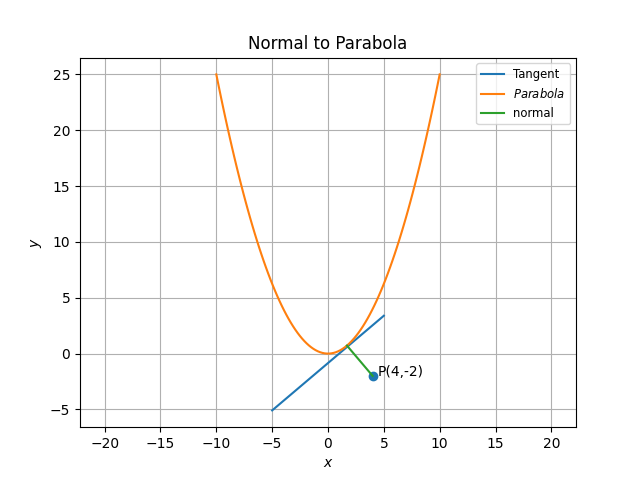
\includegraphics[width=\columnwidth]{12/6/6/4/conv/figs/12_6_6_4}
	\end{center}
\caption{}
\label{fig:12/6/6/4/conv/Fig1}
\end{figure}


\item Semi-definite Programming
\iffalse
\documentclass[12pt]{article}
\usepackage{graphicx}
\usepackage{amsmath}
\usepackage{mathtools}
\usepackage{gensymb}
\usepackage{tabularx}
\usepackage{array}
\usepackage[latin1]{inputenc}
\usepackage{fullpage}
\usepackage{color}
\usepackage{array}
\usepackage{longtable}
\usepackage{calc}
\usepackage{multirow}
\usepackage{hhline}
\usepackage{ifthen}
\usepackage{lscape}
\usepackage{float}
\usepackage{amssymb}

\newcommand{\mydet}[1]{\ensuremath{\begin{vmatrix}#1\end{vmatrix}}}
\providecommand{\brak}[1]{\ensuremath{\left(#1\right)}}
\providecommand{\norm}[1]{\left\lVert#1\right\rVert}
\providecommand{\abs}[1]{\left\vert#1\right\vert}
\newcommand{\solution}{\noindent \textbf{Solution: }}
\newcommand{\myvec}[1]{\ensuremath{\begin{pmatrix}#1\end{pmatrix}}}
\let\vec\mathbf

\def\inputGnumericTable{}

\begin{document}
\begin{center}
\textbf\large{OPTIMIZATION}

\end{center}
\section*{Excercise 6.6}

\solution
\fi
The given equation of the curve can be written as  
\begin{align}
	\label{eq:12/6/6/4/sdp/parabolaEq2}
	g\brak{\vec{x}} = \vec{x}^\top\vec{V}\vec{x} + 2\vec{u}^\top\vec{x} + f = 0 
\end{align}
where
\begin{align}
	\vec{V} = \myvec{ 1 & 0 \\ 0 & 0},\, 
	\vec{u} = \myvec{0 \\ -2},\, 
	f = 0 
\end{align}
We are given that 
\begin{align}
	\vec{h} &= \myvec{4 \\ -2}
\end{align}
This can be formulated as optimization problem as below:
\begin{align}
	\label{eq:12/6/6/4/sdp/Eq3}
	&  \min_{\vec{x}} \quad \text{f}\brak{\vec{x}} = \norm{\vec{x}-\vec{h}}^2\\
	\label{eq:12/6/6/4/sdp/Eq4}
	& \text{s.t.}\quad g\brak{\vec{x}} = \vec{x}^\top\vec{V}\vec{x} + 2\vec{u}^\top\vec{x} + f = 0  
\end{align}
Now,
\begin{align}
	\norm{\vec{x}-\vec{h}}^2 &= \norm{\vec{x}}^2 - 2\vec{h}^\top\vec{x}+\norm{\vec{h}}^2\\
	&= \vec{y}^\top\vec{C}\vec{y}
\end{align}
where,
\begin{align}
	\vec{C} = \myvec{\vec{I}&-\vec{h}\\-\vec{h}^\top& \norm{h}^2} \text{ and }
	\vec{y} = \myvec{\vec{x}\\1}
\end{align}
And equation \eqref{eq:12/6/6/4/sdp/Eq4} can be expressed as
\begin{align}
	\vec{y}^\top\vec{A}\vec{y} = 0
\end{align}
where
\begin{align}
	\vec{A} = \myvec{\vec{V}&\vec{u}\\\vec{u}^\top & f}
\end{align}
Using SDR(Semi Definite Relaxation), \eqref{eq:12/6/6/4/sdp/Eq3} can be expressed as
\begin{align}
	& \min_{\vec{X}} tr\brak{\vec{C}\vec{X}}\\
	& \text{s.t. } tr\brak{\vec{A}\vec{X}} = 0\\
	& \vec{X} \succcurlyeq \vec{0}
\end{align}
On solving it yields to the point
\begin{align}
	\vec{x} = \myvec{1.695\\0.718}
\end{align}
This is same as we obtained in Gradient Descent and Lagrange multiplier. Hence this is the required point.


















		\end{enumerate}


\item
\label{12/6/6/22}
\iffalse
\documentclass[journal,10pt,twocolumn]{article}
\usepackage{graphicx, float}
\usepackage[margin=0.5in]{geometry}
\usepackage{amsmath, bm}
\usepackage{array}
\usepackage{booktabs}
\usepackage[utf8]{inputenc}
\usepackage{amsfonts}
\usepackage{amssymb}
\usepackage{graphicx}
\usepackage{multicol}
\usepackage{tabularx}
\usepackage{hyperref}
\usepackage{mathtools}
\DeclareUnicodeCharacter{2212}{-}
\providecommand{\norm}[1]{\left\lVert#1\right\rVert}
\providecommand{\abs}[1]{\left\vert#1\right\vert}
\let\vec\mathbf
\newcommand{\myvec}[1]{\ensuremath{\begin{pmatrix}#1\end{pmatrix}}}
\newcommand{\mydet}[1]{\ensuremath{\begin{vmatrix}#1\end{vmatrix}}}
\providecommand{\brak}[1]{\ensuremath{\left(#1\right)}}
\providecommand{\lbrak}[1]{\ensuremath{\left(#1\right.}}
\providecommand{\rbrak}[1]{\ensuremath{\left.#1\right)}}
\providecommand{\sbrak}[1]{\ensuremath{{}\left[#1\right]}}
%\providecommand{\norm}[1]{\left\lVert#1\right\rVert}
%\providecommand{\sbrak}[1]{\ensuremath{{}\left[#1\right]}}
%\providecommand{\lsbrak}[1]{\ensuremath{{}\left[#1\right.}}
%\providecommand{\rsbrak}[1]{\ensuremath{{}\left.#1\right]}}
%\providecommand{\brak}[1]{\ensuremath{\left(#1\right)}}
%\providecommand{\lbrak}[1]{\ensuremath{\left(#1\right.}}
%\providecommand{\rbrak}[1]{\ensuremath{\left.#1\right)}}
%\providecommand{\cbrak}[1]{\ensuremath{\left\{#1\right\}}}
%\providecommand{\lcbrak}[1]{\ensuremath{\left\{#1\right.}}
%\providecommand{\rcbrak}[1]{\ensuremath{\left.#1\right\}}}
%\newcommand{\myvec}[1]{\ensuremath{\begin{pmatrix}#1\end{pmatrix}}}
%\let\vec\mathbf

\title{\textbf{Optimization Assignment}}
\author{Jyothsna Paluchuri \hspace{9cm} FWC22059}


\begin{document}

\maketitle
\paragraph{\textit{Problem Statement} -
\fi
Find the normal to the curve $2y+x^2=3$ passing through (2,2). 
\\
\solution 
\iffalse
:\\
(a)x+y=0  \hspace{2cm} (b)x-y=0\\ 
(c)x+y+1=0 \hspace{2cm}  (d)x-y=1\\}
\section*{\large Solution}

\begin{figure}[H]
\centering
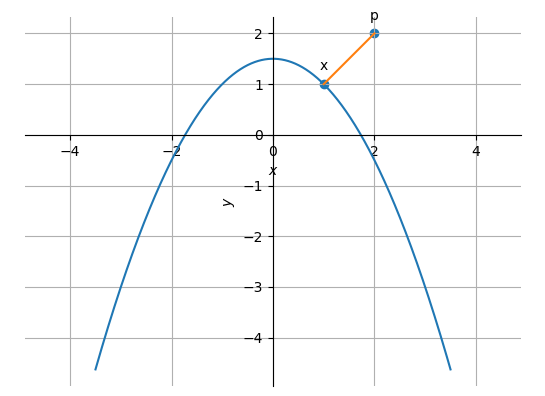
\includegraphics[width=1\columnwidth]{opt.png}
\caption{Normal to the curve $x^2+2y=3$}
\end{figure}

The given equation of parabola $x^2+2y=3$ can be written in the general quadratic form as
\begin{align}
    \vec{x}^{\top}\vec{V}\vec{x}+2\vec{u}^{\top}\vec{x}+f=0
    \end{align}
where
\fi
The parameters of the given conic are
\begin{align}
	\label{eq:12/6/6/22V_matrix}
	\vec{V} = \myvec{1 & 0\\0 & 0},
	\vec{u} = \myvec{0\\1},
	f =-3
\end{align}
If $\vec{x}$ be the point of contact on the conic, the optimization problem can be formulated as 
\begin{align}
	\label{eq:12/6/6/22/quad}
	\vec{q} = \min_{\vec{x}}\norm{\vec{x}-\vec{p}}^2
	\\
	s.t. \quad 
    \vec{x}^{\top}\vec{V}\vec{x}+2\vec{u}^{\top}\vec{x}+f=0
    \label{eq:12/6/6/22conic_quad_form}
\end{align}
%
where 
\begin{align}
	\vec{p} = \myvec{2 \\ 2}
\end{align}
Since 
\begin{align}
	\norm{\vec{x}-\vec{p}}^2 &= 
	\norm{\vec{x}}^2 - 2\vec{p}^{\top}\vec{x} + \norm{\vec{p}}^2
	\\
	&= 
\vec{y}^{\top}\vec{C}\vec{y}
\end{align}
\iffalse
\begin{center}
 Any conic of the form  $\vec{x^{\top}}\vec{V}\vec{x} + 2\vec{u^{\top}}\vec{x} + f = 0$ \end{center}
\begin{center} can be written as $\vec{x^{\top}}\vec{A}\vec{x} = 0$\end{center} 
\begin{center}
where $\vec{A} = \myvec{\vec{V}&\vec{u}\\\vec{u^{\top}}&f}$, $\vec{x} =\myvec{x\\y\\1}$
\end{center}
\begin{center}
The distance from point $\vec{p} = \myvec{2\\2}$ to the point 'x' on parabola is $\|\vec{x}-\vec{p}\|^2$
\end{center}

\begin{gather*}
	\implies 
\end{gather*}

\begin{center}
	\fi
	where
\begin{align}
	\vec{C} = \myvec{\vec{I}&-\vec{p}\\ -\vec{p}^{\top}& \norm{\vec{p}}^2}\, \vec{y} = \myvec{\vec{x}\\1}
\end{align}
and 
    \eqref{eq:12/6/6/22conic_quad_form} can be expressed as 
\begin{align}
    \vec{y}^{\top}\vec{A}\vec{y}=0,
\end{align}
where
\begin{align}
\vec{A} = \myvec{\vec{V}&\vec{u}\\\vec{u}^{\top}&f},
\end{align}
\iffalse

\begin{center}
The shortest distance is given by, min $\vec{x^{\top}}\vec{C}\vec{x}$
\end{center}
\begin{center}
such that,  $\vec{x^{\top}}\vec{A}\vec{x} = 0$
	\\ \raggedright 
\fi
	Using SDR (Semi Definite Relaxation), 
	\eqref{eq:12/6/6/22/quad}
	can be expressed as
\iffalse
	it can be rewritten as 
	\\ \centering 
\end{center}
\begin{center}
Suc that, $ 
	\fi
\begin{align}
	\min_{\vec{X}} tr\brak{\vec{C}\vec{X}}
	\\
s.t. \quad	tr\brak{\vec{A}\vec{X}} =0,
\\
 \vec{X}\succeq \vec{0}
\end{align}
\iffalse
\end{center}
\begin{center}
Here , $\vec{X}$ is a  $3\times3$ matrix of variables where
	\\ \centering $ \vec{X} = \vec{x}\vec{x^{\top}}$
\end{center}

Thus after solving we get the point on the given parabola as $\vec{x} = \myvec{1\\1}$ with the shortest distance from  $\vec{p}$
\begin{center}
	\fi
	yielding
\begin{align}
\vec{x} = \myvec{1\\1}.
\end{align}
Thus, the 
% and $\vec{p} = \myvec{2\\2}$ satisfies 
equation of the normal is
\begin{align}
	\myvec{1 &-1}\vec{x}=0
\end{align}
\iffalse
\end{center} 

\section*{\large Construction}
{
\setlength\extrarowheight{5pt}
\begin{tabular}{|c|c|c|}
	\hline
	\textbf{Symbol}&\textbf{Value}&\textbf{Description}\\[5pt]
	\hline
	$\vec{p}$&$\myvec{2 \\ 2}$&Given point through which Normal is passing\\[5pt]
	\hline
	$\vec{x}$&$\myvec{1 \\ 1}$&Foot of Normal\\[5pt]
	\hline
\end{tabular}
}

\end{document}
\fi


	\item Find the equation of the normal to the curve $x^2=4y$ and passing through the point $(1,2)$.
    \\
\solution 
		\begin{enumerate}
	\item Optimization Problem
		\\
\iffalse
\documentclass[12pt]{article}
\usepackage{graphicx}
\usepackage[none]{hyphenat}
\usepackage{graphicx}
\usepackage{listings}
\usepackage[english]{babel}
\usepackage{graphicx}
\usepackage{caption} 
\usepackage{booktabs}
\usepackage{array}
\usepackage{amssymb} % for \because
\usepackage{amsmath}   % for having text in math mode
\usepackage{extarrows} % for Row operations arrows
\usepackage{listings}
\lstset{
  frame=single,
  breaklines=true
}
\usepackage{hyperref}
  
%Following 2 lines were added to remove the blank page at the beginning
\usepackage{atbegshi}% http://ctan.org/pkg/atbegshi
\AtBeginDocument{\AtBeginShipoutNext{\AtBeginShipoutDiscard}}
\usepackage{gensymb}


%New macro definitions
\newcommand{\mydet}[1]{\ensuremath{\begin{vmatrix}#1\end{vmatrix}}}
\providecommand{\brak}[1]{\ensuremath{\left(#1\right)}}
\providecommand{\sbrak}[1]{\ensuremath{{}\left[#1\right]}}
\providecommand{\norm}[1]{\left\lVert#1\right\rVert}
\providecommand{\abs}[1]{\left\vert#1\right\vert}
\newcommand{\solution}{\noindent \textbf{Solution: }}
\newcommand{\myvec}[1]{\ensuremath{\begin{pmatrix}#1\end{pmatrix}}}
\let\vec\mathbf


\begin{document}

\begin{center}
	\title{\textbf{Quadratric Programming}}
\date{\vspace{-5ex}} %Not to print date automatically
\maketitle
\end{center}
\setcounter{page}{1}

\section{12$^{th}$ Maths - Chapter 6}
This is Problem-23 from Exercise 6.6 
\begin{enumerate}

\solution 
\fi
The given equation of the curve can be written as  
\begin{align}
	\label{eq:12/6/6/23/conv/parabolaEq2}
	g\brak{\vec{x}} = \vec{x}^T\vec{V}\vec{x} + 2\vec{u}^T\vec{x} + f = 0 
\end{align}
The given problem can be formulated as 
\begin{align}
	\label{eq:12/6/6/23/conv/Eq3}
	&  \min_{\vec{x}} \quad \text{f}\brak{\vec{x}} = \norm{\vec{x}-\vec{h}}^2\\
	\label{eq:12/6/6/23/conv/Eq4}
	& \text{s.t.}\quad g\brak{\vec{x}} = \vec{x}^T\vec{V}\vec{x} + 2\vec{u}^T\vec{x} + f = 0  
\end{align}
where
\begin{align}
	\vec{V} = \myvec{ 1 & 0 \\ 0 & 0},\,
	\vec{u} = \myvec{0 \\ -2},\, 
	f = 0,\,
	\vec{h} = \myvec{1 \\ 2}
\end{align}
The optimization problem is nonconvex. However, by relaxing the constraint in \eqref{eq:12/6/6/23/conv/Eq4} as
\begin{align}
	\label{eq:12/6/6/23/conv/Eq7}
	& g\brak{\vec{x}} = \vec{x}^T\vec{V}\vec{x} + 2\vec{u}^T\vec{x} + f \le 0  
\end{align}
the optimization problem can be made convex. Using cvxpy, input the objective function, contraints and solve. However, resultant optimal point is the given point itself. This is because, the point is inside the parabola. Looks like, this is a limitation of cvxpy.

\item Semi-definite Programming
\label{12/6/6/23}
\iffalse
\documentclass[journal,10pt,twocolumn]{article}
\usepackage{graphicx, float}
\usepackage[margin=0.5in]{geometry}
\usepackage{amsmath, bm}
\usepackage{array}
\usepackage{booktabs}
\usepackage[utf8]{inputenc}
\usepackage{amsfonts}
\usepackage{amssymb}
\usepackage{graphicx}
\usepackage{multicol}
\usepackage{tabularx}
\usepackage{hyperref}
\usepackage{mathtools}
\DeclareUnicodeCharacter{2212}{-}
\providecommand{\norm}[1]{\left\lVert#1\right\rVert}
\providecommand{\abs}[1]{\left\vert#1\right\vert}
\let\vec\mathbf
\newcommand{\myvec}[1]{\ensuremath{\begin{pmatrix}#1\end{pmatrix}}}
\newcommand{\mydet}[1]{\ensuremath{\begin{vmatrix}#1\end{vmatrix}}}
\providecommand{\brak}[1]{\ensuremath{\left(#1\right)}}
\providecommand{\lbrak}[1]{\ensuremath{\left(#1\right.}}
\providecommand{\rbrak}[1]{\ensuremath{\left.#1\right)}}
\providecommand{\sbrak}[1]{\ensuremath{{}\left[#1\right]}}
%\providecommand{\norm}[1]{\left\lVert#1\right\rVert}
%\providecommand{\sbrak}[1]{\ensuremath{{}\left[#1\right]}}
%\providecommand{\lsbrak}[1]{\ensuremath{{}\left[#1\right.}}
%\providecommand{\rsbrak}[1]{\ensuremath{{}\left.#1\right]}}
%\providecommand{\brak}[1]{\ensuremath{\left(#1\right)}}
%\providecommand{\lbrak}[1]{\ensuremath{\left(#1\right.}}
%\providecommand{\rbrak}[1]{\ensuremath{\left.#1\right)}}
%\providecommand{\cbrak}[1]{\ensuremath{\left\{#1\right\}}}
%\providecommand{\lcbrak}[1]{\ensuremath{\left\{#1\right.}}
%\providecommand{\rcbrak}[1]{\ensuremath{\left.#1\right\}}}
%\newcommand{\myvec}[1]{\ensuremath{\begin{pmatrix}#1\end{pmatrix}}}
%\let\vec\mathbf

\title{\textbf{Optimization Assignment}}
\author{Sireesha Abbavaram \hspace{9cm} FWC22060}


\begin{document}

\maketitle
\paragraph{\textit{Problem Statement} - 
\fi
Find the 
normal to the curve $x^2=4y$ passing through (1,2).
\iffalse
(a)x+y=3  \hspace{2cm} (b)x-y=3\\ 
(c)x+y=1 \hspace{2cm}  (d)x-y=1\\}

\section*{\large Solution}

\begin{figure}[H]
\centering
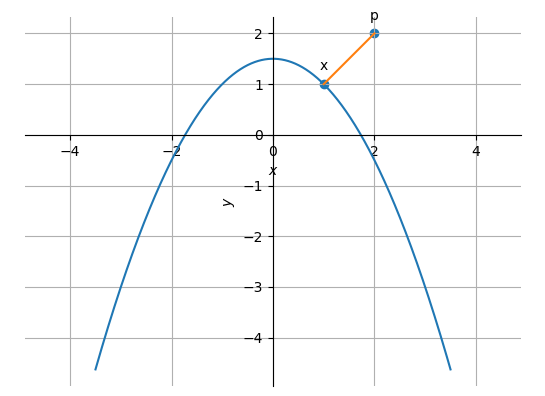
\includegraphics[width=1\columnwidth]{opt.png}
\caption{Normal to the curve $x^2=4y$}
\end{figure}

The given equation of parabola $x^2 = 4y$ can be written in the general quadratic form as
\begin{align}
    \label{eq:conic_quad_form}
    \vec{x}^{\top}\vec{V}\vec{x}+2\vec{u}^{\top}\vec{x}+f=0
    \end{align}
where
\begin{align}
	\label{eq:V_matrix}
	\vec{V} &= \myvec{1 & 0\\0 & 0},
	\\
	\label{eq:u_vector}
	\vec{u} &= \myvec{0\\-2},
	\\
	\label{eq:f_value}
	f &=0
	% ||
\end{align}
\fi
The parameters of the given conic are
\begin{align}
	\label{eq:12/6/6/23V_matrix}
	\vec{V} = \myvec{1 & 0\\0 & 0},
	\vec{u} = \myvec{0\\-2},
	f =0
\end{align}
If $\vec{x}$ be the point of contact on the conic, the optimization problem can be formulated as 
\begin{align}
	\label{eq:12/6/6/23/quad}
	\vec{q} = \min_{\vec{x}}\norm{\vec{x}-\vec{p}}^2
	\\
	s.t. \quad 
    \vec{x}^{\top}\vec{V}\vec{x}+2\vec{u}^{\top}\vec{x}+f=0
    \label{eq:12/6/6/23conic_quad_form}
\end{align}
%
where 
\begin{align}
	\vec{p} = \myvec{1 \\ 2}
\end{align}
Since 
\begin{align}
	\norm{\vec{x}-\vec{p}}^2 &= 
	\norm{\vec{x}}^2 - 2\vec{p}^{\top}\vec{x} + \norm{\vec{p}}^2
	\\
	&= 
\vec{y}^{\top}\vec{C}\vec{y}
\end{align}
	where
\begin{align}
	\vec{C} = \myvec{\vec{I}&-\vec{p}\\ -\vec{p}^{\top}& \norm{\vec{p}}^2}\, \vec{y} = \myvec{\vec{x}\\1}
\end{align}
and 
    \eqref{eq:12/6/6/23conic_quad_form} can be expressed as 
\begin{align}
    \vec{y}^{\top}\vec{A}\vec{y}=0,
\end{align}
where
\begin{align}
\vec{A} = \myvec{\vec{V}&\vec{u}\\\vec{u}^{\top}&f},
\end{align}
	Using SDR (Semi Definite Relaxation), 
	\eqref{eq:12/6/6/23/quad}
	can be expressed as
\begin{align}
	\min_{\vec{X}} tr\brak{\vec{C}\vec{X}}
	\\
s.t. \quad	tr\brak{\vec{A}\vec{X}} =0,
\\
 \vec{X}\succeq \vec{0}
\end{align}
	yielding
\begin{align}
\vec{x} = \myvec{2\\1}.
\end{align}
Thus, the 
% and $\vec{p} = \myvec{2\\2}$ satisfies 
equation of the normal is
\begin{align}
	\myvec{1 &1}\vec{x}=3
\end{align}
\iffalse
\begin{center}
 Any conic of the form  $\vec{x^{\top}}\vec{V}\vec{x} + 2\vec{u^{\top}}\vec{x} + f = 0$ \end{center}
\begin{center} can be written as $\vec{x^{\top}}\vec{A}\vec{x} = 0$\end{center} 
\begin{center}
where $\vec{A} = \myvec{\vec{V}&\vec{u}\\\vec{u^{\top}}&f}$, $\vec{x} =\myvec{x\\y\\1}$
\end{center}
\begin{center}
The distance from point $\vec{p} = \myvec{1\\2}$ to the point 'x' on parabola is $\|\vec{x}-\vec{p}\|^2$
\end{center}

\begin{gather*}
	\implies \vec{x^{\top}}\vec{x} - 2\vec{p^{\top}}\vec{x} + \|\vec{p}\|^2
\end{gather*}

\begin{center}
The above equation can be written as $\vec{x^{\top}}\vec{C}\vec{x}$
\end{center}
\begin{center}
where $\vec{C} = \myvec{\vec{I}&-\vec{p}\\ -\vec{p^{\top}}& \|\vec{p}\|^2}$, $\vec{x} = \myvec{x\\y\\1}$
\end{center}
\begin{center}
The shortest distance is given by, min $\vec{x^{\top}}\vec{C}\vec{x}$
\end{center}
\begin{center}
such that,  $\vec{x^{\top}}\vec{A}\vec{x} = 0$
	\\ \raggedright Using SDR(Semi Definite Relaxation), it can be rewritten as 
	\\ \centering min $Tr\myvec{\vec{C}\vec{X}}$
\end{center}
\begin{center}
Suc that, $ Tr\myvec{\vec{A}\vec{X}} =0,$
 $\vec{X}\ge0$
\end{center}
\begin{center}
Here , $\vec{X}$ is a  $3\times3$ matrix of variables where
	\\ \centering $ \vec{X} = \vec{x}\vec{x^{\top}}$
\end{center}



Thus after solving we get the point on the given parabola as $\vec{x} = \myvec{2\\1}$ with the shortest distance from  $\vec{p}$
\begin{center}
    Thus the points $\vec{x} = \myvec{2\\1}$ and $\vec{p} = \myvec{1\\2}$ satisfies the equation of the normal i.e. $x+y=3$
\end{center} 

\section*{\large Construction}
{
\setlength\extrarowheight{5pt}
\begin{tabular}{|c|c|c|}
	\hline
	\textbf{Symbol}&\textbf{Value}&\textbf{Description}\\[5pt]
	\hline
	$\vec{p}$&$\myvec{1 \\ 2}$&Given point through which Normal is passing\\[5pt]
	\hline
	$\vec{x}$&$\myvec{2 \\ 1}$&Foot of Normal\\[5pt]
	\hline
\end{tabular}
}

\end{document}
\fi

\item  Lagrange Multipliers
	\\
\label{12/6/6/23/lagmul}
\iffalse
\documentclass[12pt]{article}
\usepackage{graphicx}
\usepackage[none]{hyphenat}
\usepackage{graphicx}
\usepackage{listings}
\usepackage[english]{babel}
\usepackage{graphicx}
\usepackage{caption} 
\usepackage{booktabs}
\usepackage{array}
\usepackage{amssymb} % for \because
\usepackage{amsmath}   % for having text in math mode
\usepackage{extarrows} % for Row operations arrows
\usepackage{listings}
\lstset{
  frame=single,
  breaklines=true
}
\usepackage{hyperref}
  
%Following 2 lines were added to remove the blank page at the beginning
\usepackage{atbegshi}% http://ctan.org/pkg/atbegshi
\AtBeginDocument{\AtBeginShipoutNext{\AtBeginShipoutDiscard}}
\usepackage{gensymb}


%New macro definitions
\newcommand{\mydet}[1]{\ensuremath{\begin{vmatrix}#1\end{vmatrix}}}
\providecommand{\brak}[1]{\ensuremath{\left(#1\right)}}
\providecommand{\sbrak}[1]{\ensuremath{{}\left[#1\right]}}
\providecommand{\norm}[1]{\left\lVert#1\right\rVert}
\providecommand{\abs}[1]{\left\vert#1\right\vert}
\newcommand{\solution}{\noindent \textbf{Solution: }}
\newcommand{\myvec}[1]{\ensuremath{\begin{pmatrix}#1\end{pmatrix}}}
\let\vec\mathbf


\begin{document}

\begin{center}
	\title{\textbf{Quadratric Programming}}
\date{\vspace{-5ex}} %Not to print date automatically
\maketitle
\end{center}
\setcounter{page}{1}

\section{12$^{th}$ Maths - Chapter 6}
This is Problem-23 from Exercise 6.6 
\begin{enumerate}

\solution 
\fi
The given equation of the curve can be written as  
\begin{align}
	\label{eq:12/6/6/23/lagmul/parabolaEq2}
	g\brak{\vec{x}} = \vec{x}^T\vec{V}\vec{x} + 2\vec{u}^T\vec{x} + f = 0 
\end{align}
where
\begin{align}
	\label{eq:12/6/6/23/lagmul/eqV}
	\vec{V} &= \myvec{ 1 & 0 \\ 0 & 0} \\
	\label{eq:12/6/6/23/lagmul/eqU}
	\vec{u} &= \myvec{0 \\ -2} \\
	\label{eq:12/6/6/23/lagmul/eqF}
	f &= 0 
\end{align}
We are given that 
\begin{align}
	\vec{h} &= \myvec{1 \\ 2}
\end{align}
This can be formulated as optimization problem as below:
\begin{align}
	\label{eq:12/6/6/23/lagmul/Eq3}
	&  \min_{\vec{x}} \quad \text{f}\brak{\vec{x}} = \norm{\vec{x}-\vec{h}}^2\\
	\label{eq:12/6/6/23/lagmul/Eq4}
	& \text{s.t.}\quad g\brak{\vec{x}} = \vec{x}^T\vec{V}\vec{x} + 2\vec{u}^T\vec{x} + f = 0  
\end{align}
It is already proved that the optimization problem is nonconvex. The constraints throw an error when \textit{cvxpy} is used. 
We will use Lagrange multipliers method to find the optimum value. Define
\begin{align}
	H\brak{\vec{x}, \lambda} &= f\brak{\vec{x}} - \lambda g\brak{\vec{x}} 
\end{align}
and we find that 
\begin{align}
	\nabla f\brak{\vec{x}} &= 2\brak{\vec{x}-\vec{h}} \\
	\nabla g\brak{\vec{x}} &= 2\brak{\vec{V}\vec{x}+\vec{u}}
\end{align}
We have to find $\lambda \in \mathbb{R}$ such that
\begin{align}
	&\nabla H\brak{\vec{x},\lambda} = 0 \\
        \label{eq:12/6/6/23/lagmul/Eqlambda}
	&\implies 2\brak{\vec{x}-\vec{h}} - 2\lambda\brak{\vec{V}\vec{x}+\vec{u}} = 0 \\
        \label{eq:12/6/6/23/lagmul/Eqx}
	&\implies \vec{x} - \vec{h} =  \lambda\brak{\vec{V}\vec{x}+\vec{u}}   \\
	&\implies \brak{\vec{I} - \lambda\vec{V}}\vec{x} =  \lambda\vec{u}+\vec{h} \\ 
	&\implies \myvec{1-\lambda & 0 \\ 0 & 1}\vec{x} = \lambda\myvec{0 \\ -2} + \myvec{1 \\2} \\ 
        \label{eq:12/6/6/23/lagmul/EqL}
	&\implies \myvec{1-\lambda & 0 \\ 0 & 1}\vec{x} = \myvec{1 \\ -2\lambda+2}  
\end{align}
We have 2 cases to considers here.
\begin{enumerate}
\item When $\lambda \ne 1$. Writing augmented matrix,
\begin{align}
	&\myvec{1-\lambda & 0 & 1\\ 0 & 1 & -2\lambda+2} \xleftrightarrow[]{R_1 \leftarrow \frac{R_1}{1-\lambda}} \myvec{1&0&\frac{1}{1-\lambda}\\0&1&-2\lambda+2}
\end{align}
Then, we get
\begin{align}
        \label{eq:12/6/6/23/lagmul/Eqxm}
	\vec{x}_{m} &= \myvec{ \frac{1}{1-\lambda} \\ -2\lambda+2}
\end{align}
Substituting this value in \eqref{eq:12/6/6/23/lagmul/Eq4}
\begin{multline}
	\myvec{\frac{1}{1-\lambda} & -2\lambda+2}\myvec{1 & 0 \\ 0 & 0}\myvec{\frac{1}{1-\lambda} \\ -2\lambda+2} 
	+ 2\myvec{0 & -2}\myvec{\frac{1}{1-\lambda}} = 0 \\ 
	 \implies \brak{\lambda-1}^3 = -\frac{1}{8} \\ 
	 \implies \lambda = \frac{1}{2}
\end{multline}
Substituting the value of $\lambda$ in    \eqref{eq:12/6/6/23/lagmul/Eqxm}
\begin{align}
	\vec{x}_{m} &= \vec{q} = \myvec{ \frac{1}{1-\frac{1}{2}} \\ -2\brak{\frac{1}{2}}+2} \\
	&= \myvec{2 \\ 1}
\end{align}
\item When $\lambda = 1$, from \eqref{eq:12/6/6/23/lagmul/EqL},  
\begin{align}
	\myvec{0 & 0 \\ 0&1}\vec{x} = \myvec{1 \\ 0}
\end{align}
This is an invalid solution. 
\end{enumerate}
Given the point of contact $\vec{q}$, the equation to the normal is given by
\begin{align}
	&\brak{\vec{V}\vec{q}+\vec{u}}^\top\vec{R}\brak{\vec{x}-\vec{q}} = 0 \\
	&\implies \brak{\myvec{1&0\\0&0}\myvec{2\\1}+\myvec{0 \\ -2}}^\top \myvec{0&1 \\-1&0}\brak{\vec{x}-\myvec{2\\1}} =0\\
	&\implies \myvec{1&1}\vec{x} = 3 
\end{align}
The relevant figure is shown in \ref{fig:12/6/6/23/lagmul/Fig1}
\begin{figure}[!h]
	\begin{center}
		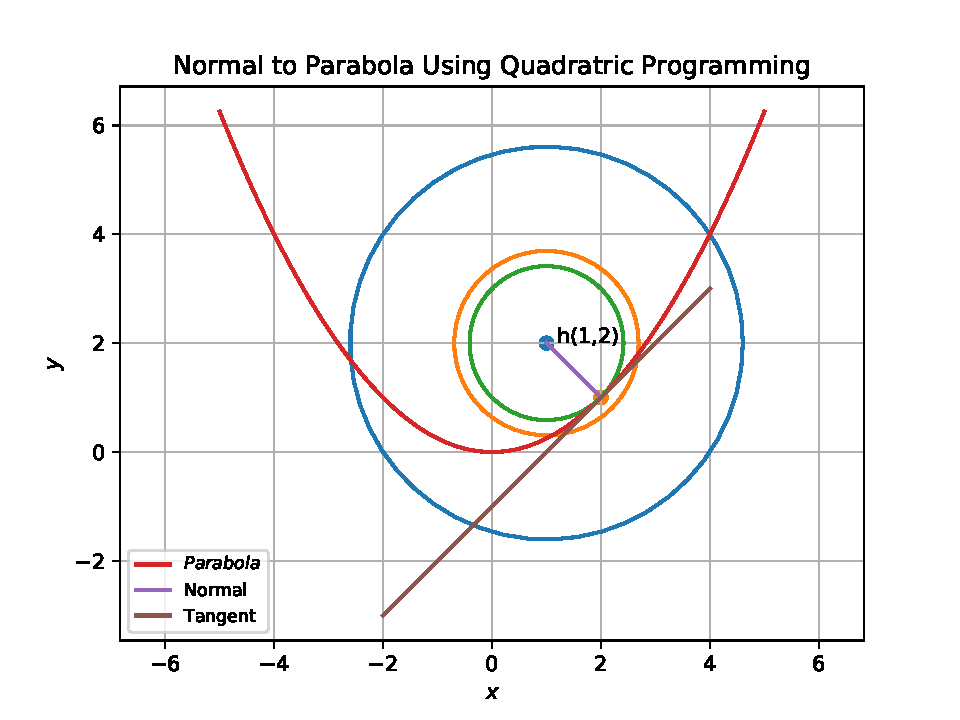
\includegraphics[width=\columnwidth]{12/6/6/23/lagmul/figs/problem23.pdf}
	\end{center}
\caption{}
\label{fig:12/6/6/23/lagmul/Fig1}
\end{figure}

		\end{enumerate}



\end{enumerate}
